\documentclass[12pt,a4paper]{article}
\usepackage[utf8]{vietnam}
\usepackage{amsmath,amssymb,amsfonts,mathrsfs}
\usepackage[left=1.5cm,right=1.5cm,top=2cm,bottom=2cm,headheight=17pt]{geometry}
\usepackage{enumitem}
\usepackage{array}
\usepackage{graphicx}
\usepackage{tikz}
\usetikzlibrary{arrows.meta,calc,patterns}
\usepackage{fancyhdr}

\pagestyle{fancy}
\fancyhf{}
\lhead{\small\textbf{HƯỚNG TỚI THPTQG 2027}}
\rhead{\small\textit{Người biên soạn: Dương Gia Bảo}}
\rfoot{\small Trang \thepage}
\renewcommand{\headrulewidth}{0.4pt}

\begin{document}

\noindent
\begin{minipage}[t]{0.40\textwidth}
    \centering
    \textbf{HƯỚNG TỚI THPTQG 2027}\\[-2pt]
    \rule{3.2cm}{0.6pt}\\[4pt]
    \textbf{ĐỀ CHÍNH THỨC}
\end{minipage}\hfill
\begin{minipage}[t]{0.58\textwidth}
    \centering
    \textbf{ĐỀ THI KHẢO SÁT CHẤT LƯỢNG}\\
    \textbf{ĐỀ SỐ 13}\\
    \textbf{Môn thi: TOÁN}\\
    \textit{\small Thời gian làm bài: 90 phút, không kể thời gian phát đề}
\end{minipage}

\vspace{0.2cm}
\noindent
\begin{minipage}[b]{0.78\textwidth}
    \textbf{Họ và tên:}\dotfill\textbf{SBD:}\makebox[3.5cm]{\dotfill}
\end{minipage}\hfill
\begin{minipage}[b]{0.20\textwidth}
    \hfill
    \setlength{\fboxrule}{0.8pt}%
    \fbox{\begin{minipage}{2.3cm}
        \centering
        \textbf{\small Mã đề thi}\\
        \textbf{0013}
    \end{minipage}}
\end{minipage}
\vspace{0.2cm}

% ==========================================
% PHẦN I
% ==========================================
\section*{\large PHẦN I. CÂU TRẮC NGHIỆM NHIỀU PHƯƠNG ÁN LỰA CHỌN}
\textit{Thí sinh trả lời từ câu 1 đến câu 12. Mỗi câu hỏi thí sinh chỉ chọn một phương án. Mỗi câu trả lời đúng được 0,25 điểm.}

\begin{enumerate}[label=\textbf{Câu \arabic*:}, leftmargin=*]

\item Cho hàm số $y = \dfrac{x^2 + 2x + 2}{x + 1}$ có đồ thị $(C)$. Khoảng cách giữa hai điểm cực trị của đồ thị $(C)$ bằng
\begin{enumerate}[label=\Alph*.]
    \item $4$.
    \item $2\sqrt{2}$.
    \item $2\sqrt{5}$.
    \item $\sqrt{10}$.
\end{enumerate}

\item Tổng tất cả các nghiệm thực của phương trình $4^x - 5\cdot 2^x + 4 = 0$ bằng
\begin{enumerate}[label=\Alph*.]
    \item $2$.
    \item $4$.
    \item $1$.
    \item $5$.
\end{enumerate}

\item Giá trị của tích phân $\displaystyle \int_1^e \left(2 + \dfrac{1}{x}\right)\mathrm{d}x$ bằng
\begin{enumerate}[label=\Alph*.]
    \item $2e + 1$.
    \item $e + 1$.
    \item $2e - 2$.
    \item $2e - 1$.
\end{enumerate}

\item Trong không gian $Oxyz$, cho điểm $A(1; 0; 2)$ và mặt phẳng $(P): x + 2y - 2z + 1 = 0$. Phương trình chính tắc của đường thẳng đi qua $A$ và vuông góc với mặt phẳng $(P)$ là
\begin{enumerate}[label=\Alph*.]
    \item $\dfrac{x - 1}{1} = \dfrac{y}{2} = \dfrac{z - 2}{2}$.
    \item $\dfrac{x - 1}{1} = \dfrac{y}{2} = \dfrac{z - 2}{-2}$.
    \item $\dfrac{x + 1}{1} = \dfrac{y}{2} = \dfrac{z + 2}{-2}$.
    \item $\dfrac{x - 1}{2} = \dfrac{y}{1} = \dfrac{z - 2}{-2}$.
\end{enumerate}

\item Một hộp chứa $6$ viên bi đỏ và $4$ viên bi xanh có kích thước và khối lượng như nhau. Lấy ngẫu nhiên đồng thời $2$ viên bi từ hộp. Xác suất để lấy được hai viên bi đều màu đỏ bằng
\begin{enumerate}[label=\Alph*.]
    \item $\dfrac{1}{3}$.
    \item $\dfrac{3}{5}$.
    \item $\dfrac{2}{5}$.
    \item $\dfrac{4}{9}$.
\end{enumerate}

\item Thời gian chờ phục vụ (đơn vị: phút) của $40$ khách hàng tại một quầy giao dịch được ghi lại trong bảng số liệu ghép nhóm sau:
\begin{center}
\begin{tabular}{|c|c|c|c|c|c|}
\hline
\textbf{Thời gian (phút)} & $[10; 20)$ & $[20; 30)$ & $[30; 40)$ & $[40; 50)$ & $[50; 60)$ \\ \hline
\textbf{Số khách hàng} & 4 & 10 & 16 & 6 & 4 \\ \hline
\end{tabular}
\end{center}
Trung vị của mẫu số liệu ghép nhóm trên bằng
\begin{enumerate}[label=\Alph*.]
    \item $32{,}50$.
    \item $35{,}00$.
    \item $33{,}75$.
    \item $34{,}25$.
\end{enumerate}

\item Cho hình chóp đều $S.ABCD$ có đáy là hình vuông cạnh $a$, cạnh bên bằng $a\sqrt{2}$. Góc giữa đường thẳng $SA$ và mặt phẳng $(ABCD)$ bằng
\begin{enumerate}[label=\Alph*.]
    \item $30^\circ$.
    \item $45^\circ$.
    \item $90^\circ$.
    \item $60^\circ$.
\end{enumerate}

\item Cho cấp số nhân $(u_n)$ có $u_1 = 2$ và công bội $q = 3$. Tổng $5$ số hạng đầu tiên của cấp số nhân đó bằng
\begin{enumerate}[label=\Alph*.]
    \item $162$.
    \item $242$.
    \item $486$.
    \item $80$.
\end{enumerate}

\item Một người gửi $200$ triệu đồng vào ngân hàng với lãi suất $6\%$/năm theo hình thức lãi kép (hết mỗi năm, tiền lãi được cộng vào vốn). Sau ít nhất bao nhiêu năm thì người đó có số tiền cả vốn lẫn lãi vượt quá $300$ triệu đồng? (giả sử lãi suất không thay đổi)
\begin{enumerate}[label=\Alph*.]
    \item $6$ năm.
    \item $8$ năm.
    \item $7$ năm.
    \item $9$ năm.
\end{enumerate}

\item Trong không gian $Oxyz$, mặt cầu có tâm $I(1; -2; 0)$ và đi qua điểm $A(3; 0; 1)$ có phương trình là
\begin{enumerate}[label=\Alph*.]
    \item $(x - 1)^2 + (y + 2)^2 + z^2 = 9$.
    \item $(x - 1)^2 + (y + 2)^2 + z^2 = 3$.
    \item $(x + 1)^2 + (y - 2)^2 + z^2 = 9$.
    \item $(x - 1)^2 + (y + 2)^2 + z^2 = 81$.
\end{enumerate}

\item Từ một tấm tôn hình vuông cạnh $12\text{ dm}$, người ta cắt bỏ bốn hình vuông nhỏ cạnh $x$ (dm) ở bốn góc rồi gập lại thành một chiếc hộp không nắp. Thể tích lớn nhất của chiếc hộp có thể tạo được bằng bao nhiêu đề-xi-mét khối?
\begin{enumerate}[label=\Alph*.]
    \item $108$.
    \item $120$.
    \item $144$.
    \item $128$.
\end{enumerate}

\item Cho hình nón có chiều cao $h = 4a$ và độ dài đường sinh $l = 5a$. Diện tích xung quanh của hình nón đã cho bằng
\begin{enumerate}[label=\Alph*.]
    \item $12\pi a^2$.
    \item $15\pi a^2$.
    \item $20\pi a^2$.
    \item $24\pi a^2$.
\end{enumerate}

\end{enumerate}

% ==========================================
% PHẦN II
% ==========================================
\vspace{0.4cm}
\section*{\large PHẦN II. CÂU TRẮC NGHIỆM ĐÚNG SAI}
\textit{Thí sinh trả lời từ câu 1 đến câu 4. Trong mỗi ý \textbf{a)}, \textbf{b)}, \textbf{c)}, \textbf{d)} ở mỗi câu, thí sinh chọn đúng hoặc sai.}

\begin{enumerate}[label=\textbf{Câu \arabic*:}, leftmargin=*]

\item Cho hàm số $y = \dfrac{x^2 - 3x + 3}{x - 2}$ có đồ thị $(C)$.
\begin{enumerate}[label=\textbf{\alph*)}]
    \item Hàm số đạt cực đại tại $x = 1$ và giá trị cực đại bằng $-1$.
    \item Giao điểm của hai đường tiệm cận của đồ thị $(C)$ là điểm $I(1; 2)$.
    \item Đường tiệm cận xiên của đồ thị $(C)$ có phương trình $y = x - 1$.
    \item Tam giác tạo bởi hai đường tiệm cận của đồ thị $(C)$ và trục hoành có diện tích bằng $\dfrac{1}{2}$.
\end{enumerate}

\item \begin{minipage}[t]{0.55\linewidth}
Một hệ thống lọc thư rác nhận thấy $30\%$ số email đến là thư rác (spam). Bộ lọc gắn nhãn spam đúng cho $95\%$ số thư spam, đồng thời gắn nhãn spam nhầm cho $4\%$ số thư bình thường. Chọn ngẫu nhiên một email.
\begin{enumerate}[label=\textbf{\alph*)}]
    \item Xác suất để email được chọn bị gắn nhãn spam bằng $0{,}325$.
    \item Nếu email bị gắn nhãn spam thì xác suất để nó thực sự là thư spam lớn hơn $90\%$.
    \item Xác suất để email được chọn vừa là thư bình thường vừa không bị gắn nhãn spam bằng $0{,}672$.
    \item Nếu email không bị gắn nhãn spam thì xác suất để nó thực sự là thư spam nhỏ hơn $2\%$.
\end{enumerate}
\end{minipage}\hfill
\begin{minipage}[t]{0.42\linewidth}
\vspace{-0.4\baselineskip}
\centering

\includegraphics[width=\linewidth, keepaspectratio]{images/de13_spam_filter.jpg}
\end{minipage}

\item \begin{minipage}[t]{0.55\linewidth}
Trong không gian $Oxyz$ (đơn vị: mét), mặt phẳng $(Oxy)$ là một mặt gương phẳng. Một tia sáng phát ra từ nguồn $A(1; 2; 3)$, chạm gương tại điểm $M$ rồi phản xạ đi qua điểm $B(7; 8; 3)$ ($A$, $B$ nằm cùng phía đối với gương). Gọi $B'$ là điểm đối xứng với $B$ qua mặt phẳng $(Oxy)$.
\begin{enumerate}[label=\textbf{\alph*)}]
    \item Tia sáng chạm gương tại điểm $M(4; 5; 0)$.
    \item Tổng quãng đường $AM + MB$ của tia sáng bằng $6\sqrt{3}\text{ m}$.
    \item Điểm $B'$ có tọa độ là $(7; 8; 3)$.
    \item Góc giữa đường thẳng $AM$ và mặt phẳng $(Oxy)$ bằng $45^\circ$.
\end{enumerate}
\end{minipage}\hfill
\begin{minipage}[t]{0.42\linewidth}
\vspace{-0.4\baselineskip}
\centering
\resizebox{\linewidth}{!}{%
\begin{tikzpicture}[>=Stealth, line join=round, line cap=round, x=0.55cm, y=0.55cm]
    % Mặt gương (phần gạch chéo bên dưới đường gương)
    \fill[pattern=north east lines, pattern color=gray!70] (-1.2,-0.45) rectangle (9.7,0);
    \draw[very thick] (-1.2,0) -- (9.7,0);
    \node[left, font=\footnotesize] at (-1.2,-0.25) {gương};

    % Các điểm trong mặt phẳng chứa tia sáng
    \coordinate (A) at (0,3);
    \coordinate (M) at (4.24,0);
    \coordinate (B) at (8.49,3);
    \coordinate (Bp) at (8.49,-3);

    % Đường đi tia sáng A -> M -> B
    \draw[very thick, blue!70!black, -{Stealth[length=2.5mm]}] (A) -- ($(A)!0.55!(M)$);
    \draw[very thick, blue!70!black] ($(A)!0.55!(M)$) -- (M);
    \draw[very thick, blue!70!black, -{Stealth[length=2.5mm]}] (M) -- ($(M)!0.6!(B)$);
    \draw[very thick, blue!70!black] ($(M)!0.6!(B)$) -- (B);

    % Đường nối ảo qua gương
    \draw[dashed, thick, gray!80!black] (M) -- (Bp);
    \draw[dashed, thin, gray!70] (B) -- (Bp);
    \draw[thin] (8.49,0.4) -- (8.09,0.4) -- (8.09,0);

    % Điểm mốc
    \filldraw[fill=blue!25, draw=black, thick] (A) circle (2.2pt) node[above left, fill=white, inner sep=1.2pt] {$A$};
    \filldraw[fill=orange!80!red, draw=black, thick] (M) circle (2.2pt) node[above, fill=white, inner sep=1.2pt] {$M$};
    \filldraw[fill=blue!25, draw=black, thick] (B) circle (2.2pt) node[above right, fill=white, inner sep=1.2pt] {$B$};
    \filldraw[fill=white, draw=black, thick] (Bp) circle (2.2pt) node[below right, fill=white, inner sep=1.2pt] {$B'$};
\end{tikzpicture}%
}
\end{minipage}

\item Thời gian giao hàng (đơn vị: phút) của $50$ đơn hàng tại một cửa hàng được thống kê trong bảng số liệu ghép nhóm sau:
\begin{center}
\begin{tabular}{|c|c|c|c|c|c|}
\hline
\textbf{Thời gian (phút)} & $[0; 5)$ & $[5; 10)$ & $[10; 15)$ & $[15; 20)$ & $[20; 25)$ \\ \hline
\textbf{Số đơn hàng} & 5 & 12 & 17 & 10 & 6 \\ \hline
\end{tabular}
\end{center}
\begin{enumerate}[label=\textbf{\alph*)}]
    \item Thời gian giao hàng trung bình của mẫu số liệu ghép nhóm trên là $12{,}5$ phút.
    \item Tứ phân vị thứ nhất của mẫu số liệu ghép nhóm trên bằng $8{,}5$.
    \item Tứ phân vị thứ ba của mẫu số liệu ghép nhóm trên bằng $16{,}75$.
    \item Phương sai của mẫu số liệu ghép nhóm trên bằng $33$.
\end{enumerate}

\end{enumerate}

% ==========================================
% PHẦN III
% ==========================================
\vspace{0.4cm}
\section*{\large PHẦN III. CÂU TRẮC NGHIỆM TRẢ LỜI NGẮN}
\textit{Thí sinh trả lời từ câu 1 đến câu 6. Mỗi câu trả lời đúng được 0,5 điểm.}

\begin{enumerate}[label=\textbf{Câu \arabic*:}, leftmargin=*]

\item Cho hình lập phương $ABCD.A'B'C'D'$ có cạnh bằng $6\text{ dm}$. Khoảng cách giữa hai đường thẳng $AC$ và $BD'$ bằng bao nhiêu đề-xi-mét? (kết quả làm tròn đến hàng phần mười).

\item \begin{minipage}[t]{0.55\linewidth}
Một mặt cắt của mái vòm kính được giới hạn bởi parabol $y = 4 - x^2$ và đường thẳng $y = x + 2$ (đơn vị trên các trục là mét). Phần mặt cắt giới hạn bởi parabol và đường thẳng (phần gạch chéo trong hình vẽ) được lắp kính cường lực. Diện tích phần được lắp kính cường lực bằng bao nhiêu mét vuông?
\end{minipage}\hfill
\begin{minipage}[t]{0.42\linewidth}
\vspace{-0.4\baselineskip}
\centering
\resizebox{\linewidth}{!}{%
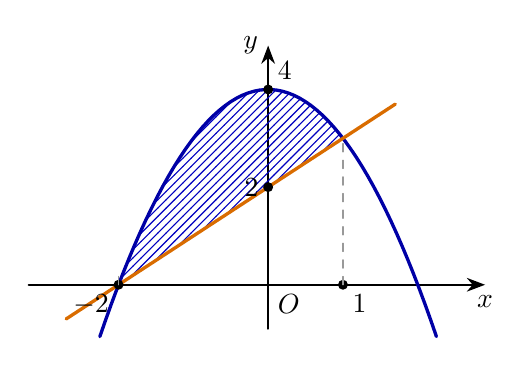
\begin{tikzpicture}[>=Stealth, x=0.95cm, y=0.62cm, line join=round, line cap=round]
    % Trục tọa độ
    \draw[->, thick] (-3.2,0) -- (2.9,0) node[below] {$x$};
    \draw[->, thick] (0,-0.9) -- (0,4.9) node[left] {$y$};
    \node[below right] at (0,0) {$O$};

    % Miền gạch chéo giữa parabol và đường thẳng
    \fill[pattern=north east lines, pattern color=blue!75!black, domain=-2:1, samples=50]
        plot (\x, {4 - \x*\x}) -- cycle;

    % Parabol và đường thẳng
    \draw[very thick, blue!65!black, domain=-2.25:2.25, samples=60] plot (\x, {4 - \x*\x});
    \draw[very thick, orange!85!black] (-2.7,-0.7) -- (1.7,3.7);

    % Giao điểm và mốc trên trục
    \fill (-2,0) circle (1.8pt) node[below left] {$-2$};
    \fill (1,0) circle (1.8pt) node[below right] {$1$};
    \fill (0,4) circle (1.8pt) node[above right] {$4$};
    \fill (0,2) circle (1.8pt) node[left] {$2$};
    \draw[dashed, thin, gray!80] (1,0) -- (1,3);
    \draw[dashed, thin, gray!80] (-2,0) -- (-2,0.2);
\end{tikzpicture}%
}
\end{minipage}

\item \begin{minipage}[t]{0.58\linewidth}
Một nhà máy cần sản xuất các lon nước dạng hình trụ (có đáy và nắp) có thể tích bằng $1000\text{ cm}^3$. Để tiết kiệm vật liệu, diện tích toàn phần của lon nước phải nhỏ nhất. Diện tích toàn phần nhỏ nhất đó bằng bao nhiêu xăng-ti-mét vuông? (kết quả làm tròn đến hàng phần mười, bỏ qua độ dày vỏ lon).
\end{minipage}\hfill
\begin{minipage}[t]{0.38\linewidth}
\vspace{-0.4\baselineskip}
\centering
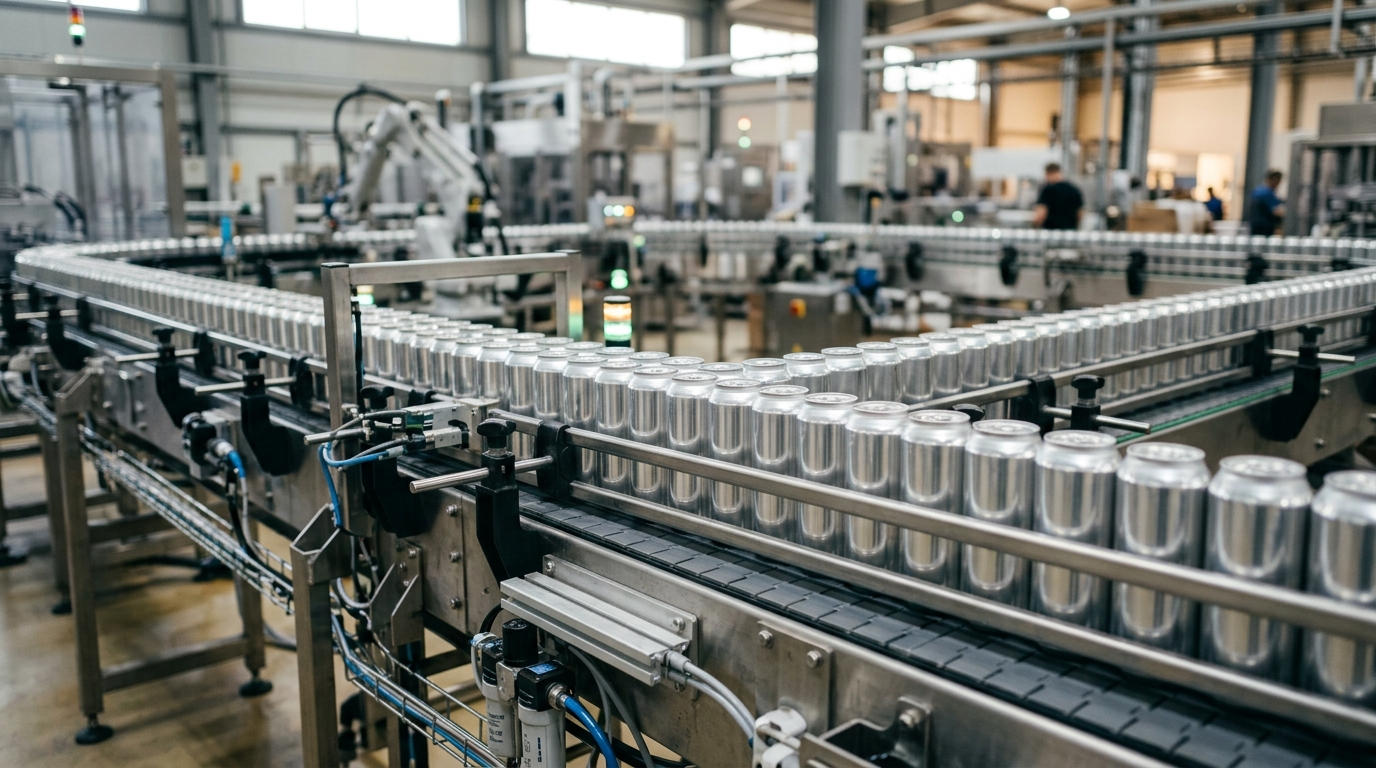
\includegraphics[width=\linewidth, keepaspectratio]{images/de13_beverage_can.jpg}
\end{minipage}

\item Trong không gian $Oxyz$ (đơn vị: ki-lô-mét), hai đường ống dẫn khí ngầm đi theo hai đường thẳng chéo nhau
\[
d_1: \dfrac{x - 1}{1} = \dfrac{y + 1}{2} = \dfrac{z}{2}, \qquad d_2: \dfrac{x - 2}{2} = \dfrac{y}{1} = \dfrac{z - 6}{-2}.
\]
Khoảng cách ngắn nhất giữa hai đường ống bằng bao nhiêu ki-lô-mét?

\item Một bài kiểm tra trắc nghiệm gồm $10$ câu, mỗi câu có $4$ phương án trả lời, trong đó chỉ có đúng một phương án đúng. Một học sinh không biết kiến thức nên chọn ngẫu nhiên một phương án ở mỗi câu. Xác suất để học sinh đó trả lời đúng ít nhất $2$ câu bằng bao nhiêu? (kết quả làm tròn đến hàng phần trăm).

\item Một chất điểm chuyển động thẳng với vận tốc $v(t) = t^2 - 4t + 3$ (đơn vị: m/s), trong đó $t$ là thời gian tính bằng giây. Quãng đường chất điểm đi được trong $4$ giây đầu tiên bằng bao nhiêu mét?

\end{enumerate}

% ==========================================
% BẢNG ĐÁP ÁN TỔNG HỢP (BẮT BUỘC TRANG MỚI)
% ==========================================
\newpage
\begin{center}
    {\Large\textbf{BẢNG ĐÁP ÁN TỔNG HỢP}}\\[4pt]
    \textbf{ĐỀ SỐ 13 - MÔN: TOÁN}
\end{center}
\vspace{0.3cm}

\noindent\textbf{\large PHẦN I. CÂU TRẮC NGHIỆM NHIỀU PHƯƠNG ÁN LỰA CHỌN}
\begin{center}
\renewcommand{\arraystretch}{1.25}
\begin{tabular}{|c|c|c|c|c|c|c|c|c|c|c|c|}
\hline
\textbf{1} & \textbf{2} & \textbf{3} & \textbf{4} & \textbf{5} & \textbf{6} & \textbf{7} & \textbf{8} & \textbf{9} & \textbf{10} & \textbf{11} & \textbf{12} \\ \hline
\textbf{C} & \textbf{A} & \textbf{D} & \textbf{B} & \textbf{A} & \textbf{C} & \textbf{D} & \textbf{B} & \textbf{C} & \textbf{A} & \textbf{D} & \textbf{B} \\ \hline
\end{tabular}
\end{center}

\vspace{0.3cm}
\noindent\textbf{\large PHẦN II. CÂU TRẮC NGHIỆM ĐÚNG SAI}
\begin{center}
\renewcommand{\arraystretch}{1.25}
\begin{tabular}{|c|c|c|c|c|}
\hline
\textbf{Câu} & \textbf{Ý a)} & \textbf{Ý b)} & \textbf{Ý c)} & \textbf{Ý d)} \\ \hline
\textbf{Câu 1} & Đ & S & Đ & Đ \\ \hline
\textbf{Câu 2} & S & Đ & Đ & S \\ \hline
\textbf{Câu 3} & Đ & Đ & S & S \\ \hline
\textbf{Câu 4} & Đ & S & Đ & Đ \\ \hline
\end{tabular}
\end{center}

\vspace{0.3cm}
\noindent\textbf{\large PHẦN III. CÂU TRẮC NGHIỆM TRẢ LỜI NGẮN}
\begin{center}
\renewcommand{\arraystretch}{1.25}
\begin{tabular}{|c|c|c|c|c|c|}
\hline
\textbf{Câu 1} & \textbf{Câu 2} & \textbf{Câu 3} & \textbf{Câu 4} & \textbf{Câu 5} & \textbf{Câu 6} \\ \hline
2,4 & 4,5 & 553,6 & 2 & 0,76 & 4 \\ \hline
\end{tabular}
\end{center}

% ==========================================
% HƯỚNG DẪN GIẢI CHI TIẾT
% ==========================================
\newpage
\begin{center}
    {\Large\textbf{HƯỚNG DẪN GIẢI CHI TIẾT}}\\[4pt]
    \textbf{ĐỀ SỐ 13 - MÔN: TOÁN}
\end{center}
\vspace{0.3cm}

\section*{\large PHẦN I. CÂU TRẮC NGHIỆM NHIỀU PHƯƠNG ÁN LỰA CHỌN}

\noindent\textbf{Câu 1.} Ta có $y = x + 1 + \dfrac{1}{x + 1}$, suy ra $y' = 1 - \dfrac{1}{(x + 1)^2}$.\\
Cho $y' = 0 \iff (x + 1)^2 = 1 \iff x = 0$ hoặc $x = -2$.\\
Hai điểm cực trị là $A(0; 2)$ và $B(-2; -2)$. Khoảng cách:
\[
AB = \sqrt{(0 + 2)^2 + (2 + 2)^2} = \sqrt{20} = 2\sqrt{5}.
\]
\textbf{Chọn C.}

\vspace{0.25cm}
\noindent\textbf{Câu 2.} Đặt $u = 2^x > 0$, phương trình trở thành $u^2 - 5u + 4 = 0 \iff u = 1$ hoặc $u = 4$.\\
Với $u = 1 \Rightarrow x = 0$; với $u = 4 \Rightarrow x = 2$. Tổng các nghiệm bằng $0 + 2 = 2$.\\
\textbf{Chọn A.}

\vspace{0.25cm}
\noindent\textbf{Câu 3.}
\[
\int_1^e \left(2 + \dfrac{1}{x}\right)\mathrm{d}x = \Big[2x + \ln x\Big]_1^e = (2e + 1) - (2 + 0) = 2e - 1.
\]
\textbf{Chọn D.}

\vspace{0.25cm}
\noindent\textbf{Câu 4.} Mặt phẳng $(P)$ có vectơ pháp tuyến $\vec{n} = (1; 2; -2)$. Đường thẳng vuông góc với $(P)$ nhận $\vec{n}$ làm vectơ chỉ phương, đi qua $A(1; 0; 2)$ nên có phương trình
\[
\dfrac{x - 1}{1} = \dfrac{y}{2} = \dfrac{z - 2}{-2}.
\]
\textbf{Chọn B.}

\vspace{0.25cm}
\noindent\textbf{Câu 5.} Số cách lấy $2$ viên bi bất kì: $C_{10}^2 = 45$. Số cách lấy $2$ viên bi đỏ: $C_6^2 = 15$.\\
Xác suất cần tìm là $\dfrac{15}{45} = \dfrac{1}{3}$.\\
\textbf{Chọn A.}

\vspace{0.25cm}
\noindent\textbf{Câu 6.} Cỡ mẫu $n = 40$, $\dfrac{n}{2} = 20$. Tần số tích lũy: $4;\ 14;\ 30;\ 36;\ 40$.\\
Nhóm chứa trung vị là $[30; 40)$ với $L = 30$, $h = 10$, $f = 16$, tần số tích lũy nhóm trước $cf = 14$:
\[
M_e = 30 + \dfrac{20 - 14}{16}\cdot 10 = 30 + 3{,}75 = 33{,}75.
\]
\textbf{Chọn C.}

\vspace{0.25cm}
\noindent\textbf{Câu 7.} Gọi $O$ là tâm hình vuông $ABCD$ thì $SO \perp (ABCD)$ và $OA = \dfrac{a\sqrt{2}}{2}$. Góc giữa $SA$ và $(ABCD)$ là $\widehat{SAO}$:
\[
\cos\widehat{SAO} = \dfrac{OA}{SA} = \dfrac{a\sqrt{2}/2}{a\sqrt{2}} = \dfrac{1}{2} \implies \widehat{SAO} = 60^\circ.
\]
\textbf{Chọn D.}

\vspace{0.25cm}
\noindent\textbf{Câu 8.}
\[
S_5 = u_1 \cdot \dfrac{q^5 - 1}{q - 1} = 2\cdot \dfrac{3^5 - 1}{3 - 1} = 242.
\]
\textbf{Chọn B.}

\vspace{0.25cm}
\noindent\textbf{Câu 9.} Sau $n$ năm, số tiền là $200\cdot (1{,}06)^n$ (triệu đồng). Ta cần $200\cdot (1{,}06)^n > 300 \iff n > \log_{1{,}06} 1{,}5 \approx 6{,}96$.\\
Vậy $n$ nguyên nhỏ nhất là $7$ (kiểm tra: $200\cdot 1{,}06^6 \approx 283{,}7 < 300$; $200\cdot 1{,}06^7 \approx 300{,}7 > 300$).\\
\textbf{Chọn C.}

\vspace{0.25cm}
\noindent\textbf{Câu 10.} Bán kính $R = IA = \sqrt{(3 - 1)^2 + (0 + 2)^2 + (1 - 0)^2} = \sqrt{9} = 3$. Phương trình mặt cầu: $(x - 1)^2 + (y + 2)^2 + z^2 = 9$.\\
\textbf{Chọn A.}

\vspace{0.25cm}
\noindent\textbf{Câu 11.} Đáy hộp là hình vuông cạnh $12 - 2x$, chiều cao $x$ với $0 < x < 6$:
\[
V(x) = x(12 - 2x)^2, \quad V'(x) = (12 - 2x)(12 - 6x).
\]
$V'(x) = 0 \iff x = 2$ (loại $x = 6$). Lập bảng biến thiên, $V$ đạt cực đại tại $x = 2$ với $V(2) = 2\cdot 8^2 = 128\text{ dm}^3$.\\
\textbf{Chọn D.}

\vspace{0.25cm}
\noindent\textbf{Câu 12.} Bán kính đáy $R = \sqrt{l^2 - h^2} = \sqrt{25a^2 - 16a^2} = 3a$. Diện tích xung quanh:
\[
S_{xq} = \pi R l = \pi\cdot 3a\cdot 5a = 15\pi a^2.
\]
\textbf{Chọn B.}

% ==========================================
\vspace{0.4cm}
\section*{\large PHẦN II. CÂU TRẮC NGHIỆM ĐÚNG SAI}

\noindent\textbf{Câu 1.} Ta có $y = x - 1 + \dfrac{1}{x - 2}$, $y' = 1 - \dfrac{1}{(x - 2)^2}$. Cho $y' = 0 \iff x = 1$ hoặc $x = 3$.\\
Với $x < 1$: $y' > 0$; với $1 < x < 2$: $y' < 0$; với $2 < x < 3$: $y' < 0$; với $x > 3$: $y' > 0$.\\
Hàm số đạt cực đại tại $x = 1$ với $y(1) = -1$ và đạt cực tiểu tại $x = 3$ với $y(3) = 3$.\\
$\implies$ \textbf{a) ĐÚNG.}

Tiệm cận đứng $x = 2$, tiệm cận xiên $y = x - 1$. Giao điểm hai tiệm cận là $I(2; 1) \ne (1; 2)$.\\
$\implies$ \textbf{b) SAI.}

Do $y = x - 1 + \dfrac{1}{x - 2}$ nên tiệm cận xiên là $y = x - 1$.\\
$\implies$ \textbf{c) ĐÚNG.}

Hai tiệm cận cắt trục hoành lần lượt tại $(2; 0)$ và $(1; 0)$. Tam giác có ba đỉnh $I(2; 1)$, $(2; 0)$, $(1; 0)$ vuông tại $(2; 0)$ với hai cạnh góc vuông bằng $1$, nên diện tích bằng $\dfrac{1}{2}\cdot 1\cdot 1 = \dfrac{1}{2}$.\\
$\implies$ \textbf{d) ĐÚNG.}

\vspace{0.3cm}
\noindent\textbf{Câu 2.} Gọi $S$: "email là spam", $T$: "email bị gắn nhãn spam". Ta có $P(S) = 0{,}3$, $P(\overline{S}) = 0{,}7$, $P(T|S) = 0{,}95$, $P(T|\overline{S}) = 0{,}04$.
\[
P(T) = 0{,}3\cdot 0{,}95 + 0{,}7\cdot 0{,}04 = 0{,}285 + 0{,}028 = 0{,}313 \ne 0{,}325.
\]
$\implies$ \textbf{a) SAI.}

\[
P(S|T) = \dfrac{0{,}285}{0{,}313} \approx 0{,}9105 > 0{,}9.
\]
$\implies$ \textbf{b) ĐÚNG.}

\[
P(\overline{S}\cap\overline{T}) = P(\overline{S})\cdot P(\overline{T}|\overline{S}) = 0{,}7\cdot 0{,}96 = 0{,}672.
\]
$\implies$ \textbf{c) ĐÚNG.}

\[
P(S|\overline{T}) = \dfrac{0{,}3\cdot 0{,}05}{1 - 0{,}313} = \dfrac{0{,}015}{0{,}687} \approx 0{,}0218 = 2{,}18\% > 2\%.
\]
$\implies$ \textbf{d) SAI.}

\vspace{0.3cm}
\noindent\textbf{Câu 3.} Điểm đối xứng của $B(7; 8; 3)$ qua $(Oxy)$ là $B'(7; 8; -3)$. Do đó \textbf{c) SAI.}

Theo định luật phản xạ, $M$ là giao điểm của đường thẳng $AB'$ với mặt phẳng $(Oxy)$. Ta có $\overrightarrow{AB'} = (6; 6; -6)$, phương trình $AB'$: $\begin{cases} x = 1 + 6t \\ y = 2 + 6t \\ z = 3 - 6t \end{cases}$.\\
$z = 0 \iff t = \dfrac{1}{2}$, suy ra $M(4; 5; 0)$.\\
$\implies$ \textbf{a) ĐÚNG.}

Vì $MB = MB'$ nên $AM + MB = AM + MB' = AB' = \sqrt{6^2 + 6^2 + 6^2} = 6\sqrt{3}\text{ m}$.\\
$\implies$ \textbf{b) ĐÚNG.}

Ta có $\overrightarrow{AM} = (3; 3; -3)$, vectơ pháp tuyến của $(Oxy)$ là $\vec{k} = (0; 0; 1)$:
\[
\sin(AM, (Oxy)) = \dfrac{|-3|}{3\sqrt{3}} = \dfrac{1}{\sqrt{3}} \approx 0{,}577 \ne \sin 45^\circ.
\]
Do đó góc giữa $AM$ và $(Oxy)$ khác $45^\circ$ (xấp xỉ $35{,}3^\circ$).\\
$\implies$ \textbf{d) SAI.}

\vspace{0.3cm}
\noindent\textbf{Câu 4.} Giá trị đại diện các nhóm: $2{,}5;\ 7{,}5;\ 12{,}5;\ 17{,}5;\ 22{,}5$.
\[
\overline{x} = \dfrac{5\cdot 2{,}5 + 12\cdot 7{,}5 + 17\cdot 12{,}5 + 10\cdot 17{,}5 + 6\cdot 22{,}5}{50} = \dfrac{625}{50} = 12{,}5.
\]
$\implies$ \textbf{a) ĐÚNG.}

Tần số tích lũy: $5;\ 17;\ 34;\ 44;\ 50$.\\
$Q_1$: $\dfrac{n}{4} = 12{,}5$ thuộc nhóm $[5; 10)$:
\[
Q_1 = 5 + \dfrac{12{,}5 - 5}{12}\cdot 5 = 5 + 3{,}125 = 8{,}125 \ne 8{,}5.
\]
$\implies$ \textbf{b) SAI.}

$Q_3$: $\dfrac{3n}{4} = 37{,}5$ thuộc nhóm $[15; 20)$:
\[
Q_3 = 15 + \dfrac{37{,}5 - 34}{10}\cdot 5 = 15 + 1{,}75 = 16{,}75.
\]
$\implies$ \textbf{c) ĐÚNG.}

Phương sai:
\[
s^2 = \dfrac{5(10)^2 + 12(5)^2 + 17\cdot 0 + 10(5)^2 + 6(10)^2}{50} = \dfrac{500 + 300 + 0 + 250 + 600}{50} = 33.
\]
$\implies$ \textbf{d) ĐÚNG.}

% ==========================================
\vspace{0.4cm}
\section*{\large PHẦN III. CÂU TRẮC NGHIỆM TRẢ LỜI NGẮN}

\noindent\textbf{Câu 1.} Chọn hệ trục $Oxyz$ với $A(0; 0; 0)$, $B(6; 0; 0)$, $D(0; 6; 0)$, $A'(0; 0; 6)$, suy ra $C(6; 6; 0)$, $D'(0; 6; 6)$.\\
Đường thẳng $AC$ có $\vec{u}_1 = (6; 6; 0)$, đường thẳng $BD'$ có $\vec{u}_2 = (-6; 6; 6)$ và $\overrightarrow{AB} = (6; 0; 0)$.
\[
[\vec{u}_1, \vec{u}_2] = (36; -36; 72), \qquad d(AC, BD') = \dfrac{|\overrightarrow{AB}\cdot[\vec{u}_1, \vec{u}_2]|}{|[\vec{u}_1, \vec{u}_2]|} = \dfrac{216}{36\sqrt{6}} = \sqrt{6} \approx 2{,}449.
\]
Làm tròn: $2{,}4$.\\
\textbf{Đáp số: 2,4.}

\vspace{0.3cm}
\noindent\textbf{Câu 2.} Hoành độ giao điểm: $4 - x^2 = x + 2 \iff x^2 + x - 2 = 0 \iff x = -2$ hoặc $x = 1$.\\
Trên $[-2; 1]$ ta có $4 - x^2 \ge x + 2$, do đó
\[
S = \int_{-2}^{1} \left[(4 - x^2) - (x + 2)\right]\mathrm{d}x = \int_{-2}^{1} (-x^2 - x + 2)\,\mathrm{d}x = \left[-\dfrac{x^3}{3} - \dfrac{x^2}{2} + 2x\right]_{-2}^{1} = \dfrac{7}{6} + \dfrac{10}{3} = \dfrac{9}{2}.
\]
\textbf{Đáp số: 4,5.}

\vspace{0.3cm}
\noindent\textbf{Câu 3.} Gọi $r$, $h$ là bán kính đáy và chiều cao ($\text{cm}$). Từ $\pi r^2 h = 1000$ suy ra $h = \dfrac{1000}{\pi r^2}$.\\
Diện tích toàn phần:
\[
S(r) = 2\pi r^2 + 2\pi r h = 2\pi r^2 + \dfrac{2000}{r}, \quad S'(r) = 4\pi r - \dfrac{2000}{r^2}.
\]
$S'(r) = 0 \iff r^3 = \dfrac{500}{\pi} \iff r \approx 5{,}419$. $S(r)$ đạt giá trị nhỏ nhất tại $r$ này (khi đó $h = 2r$):
\[
S_{\min} = 6\pi r^2 \approx 6\pi\cdot 29{,}37 \approx 553{,}6\text{ cm}^2.
\]
\textbf{Đáp số: 553,6.}

\vspace{0.3cm}
\noindent\textbf{Câu 4.} $d_1$ đi qua $M_1(1; -1; 0)$ có $\vec{u}_1 = (1; 2; 2)$; $d_2$ đi qua $M_2(2; 0; 6)$ có $\vec{u}_2 = (2; 1; -2)$.
\[
[\vec{u}_1, \vec{u}_2] = (-6; 6; -3), \quad \overrightarrow{M_1M_2} = (1; 1; 6).
\]
\[
d(d_1, d_2) = \dfrac{|\overrightarrow{M_1M_2}\cdot[\vec{u}_1, \vec{u}_2]|}{|[\vec{u}_1, \vec{u}_2]|} = \dfrac{|-6 + 6 - 18|}{\sqrt{36 + 36 + 9}} = \dfrac{18}{9} = 2.
\]
\textbf{Đáp số: 2.}

\vspace{0.3cm}
\noindent\textbf{Câu 5.} Gọi $X$ là số câu trả lời đúng, $X \sim B(10; 0{,}25)$.
\[
P(X \ge 2) = 1 - P(X = 0) - P(X = 1) = 1 - (0{,}75)^{10} - 10\cdot 0{,}25\cdot (0{,}75)^9 \approx 1 - 0{,}0563 - 0{,}1877 = 0{,}756.
\]
Làm tròn: $0{,}76$.\\
\textbf{Đáp số: 0,76.}

\vspace{0.3cm}
\noindent\textbf{Câu 6.} $v(t) = (t - 1)(t - 3)$ nên $v \ge 0$ trên $[0; 1]$, $v \le 0$ trên $[1; 3]$, $v \ge 0$ trên $[3; 4]$. Quãng đường:
\[
s = \int_0^4 |v(t)|\,\mathrm{d}t = \int_0^1 v\,\mathrm{d}t - \int_1^3 v\,\mathrm{d}t + \int_3^4 v\,\mathrm{d}t.
\]
Nguyên hàm $F(t) = \dfrac{t^3}{3} - 2t^2 + 3t$ có $F(0) = 0$, $F(1) = \dfrac{4}{3}$, $F(3) = 0$, $F(4) = \dfrac{4}{3}$. Do đó
\[
s = \dfrac{4}{3} + \dfrac{4}{3} + \dfrac{4}{3} = 4\text{ m}.
\]
\textbf{Đáp số: 4.}

\end{document}
